% !TEX root = comparison.tex
\section{Experiments}~\label{setup}

Two recent data analyses motivated the setup of this experiment. The first one arises from an analysis of US flight traffic data, and a finding related to how wind direction affects the efficiency of an airport.  The second one arose during the review of a paper claiming that it was impossible to statistically test for differences in center between two samples where sample size was small and from a non-normal population, with application to studying toxic waste sites. Using lineups containing dotplots we found it was possible to detect a difference, and we were curious to see if other display types (density, histogram, boxplot) might compare with dotplots.

%We want two discuss two applications, in which we are making use of lineups to compare competing designs. in the second example we are interested in visualizing mean shifts between two distributions.  

\subsection{Data Collection}
Data for both studies was collected using Amazon's Mechanical Turk (MTurk) service. 
The website for the second study is available at \url{http://www.public.iastate.edu/~mahbub/feedback_turk5/homepage.html}. Figure \ref{fig:screen} shows a screen shot of the website's layout for a dotplot lineup.

\begin{figure}[htbp] %  figure placement: here, top, bottom, or page
   \centering
   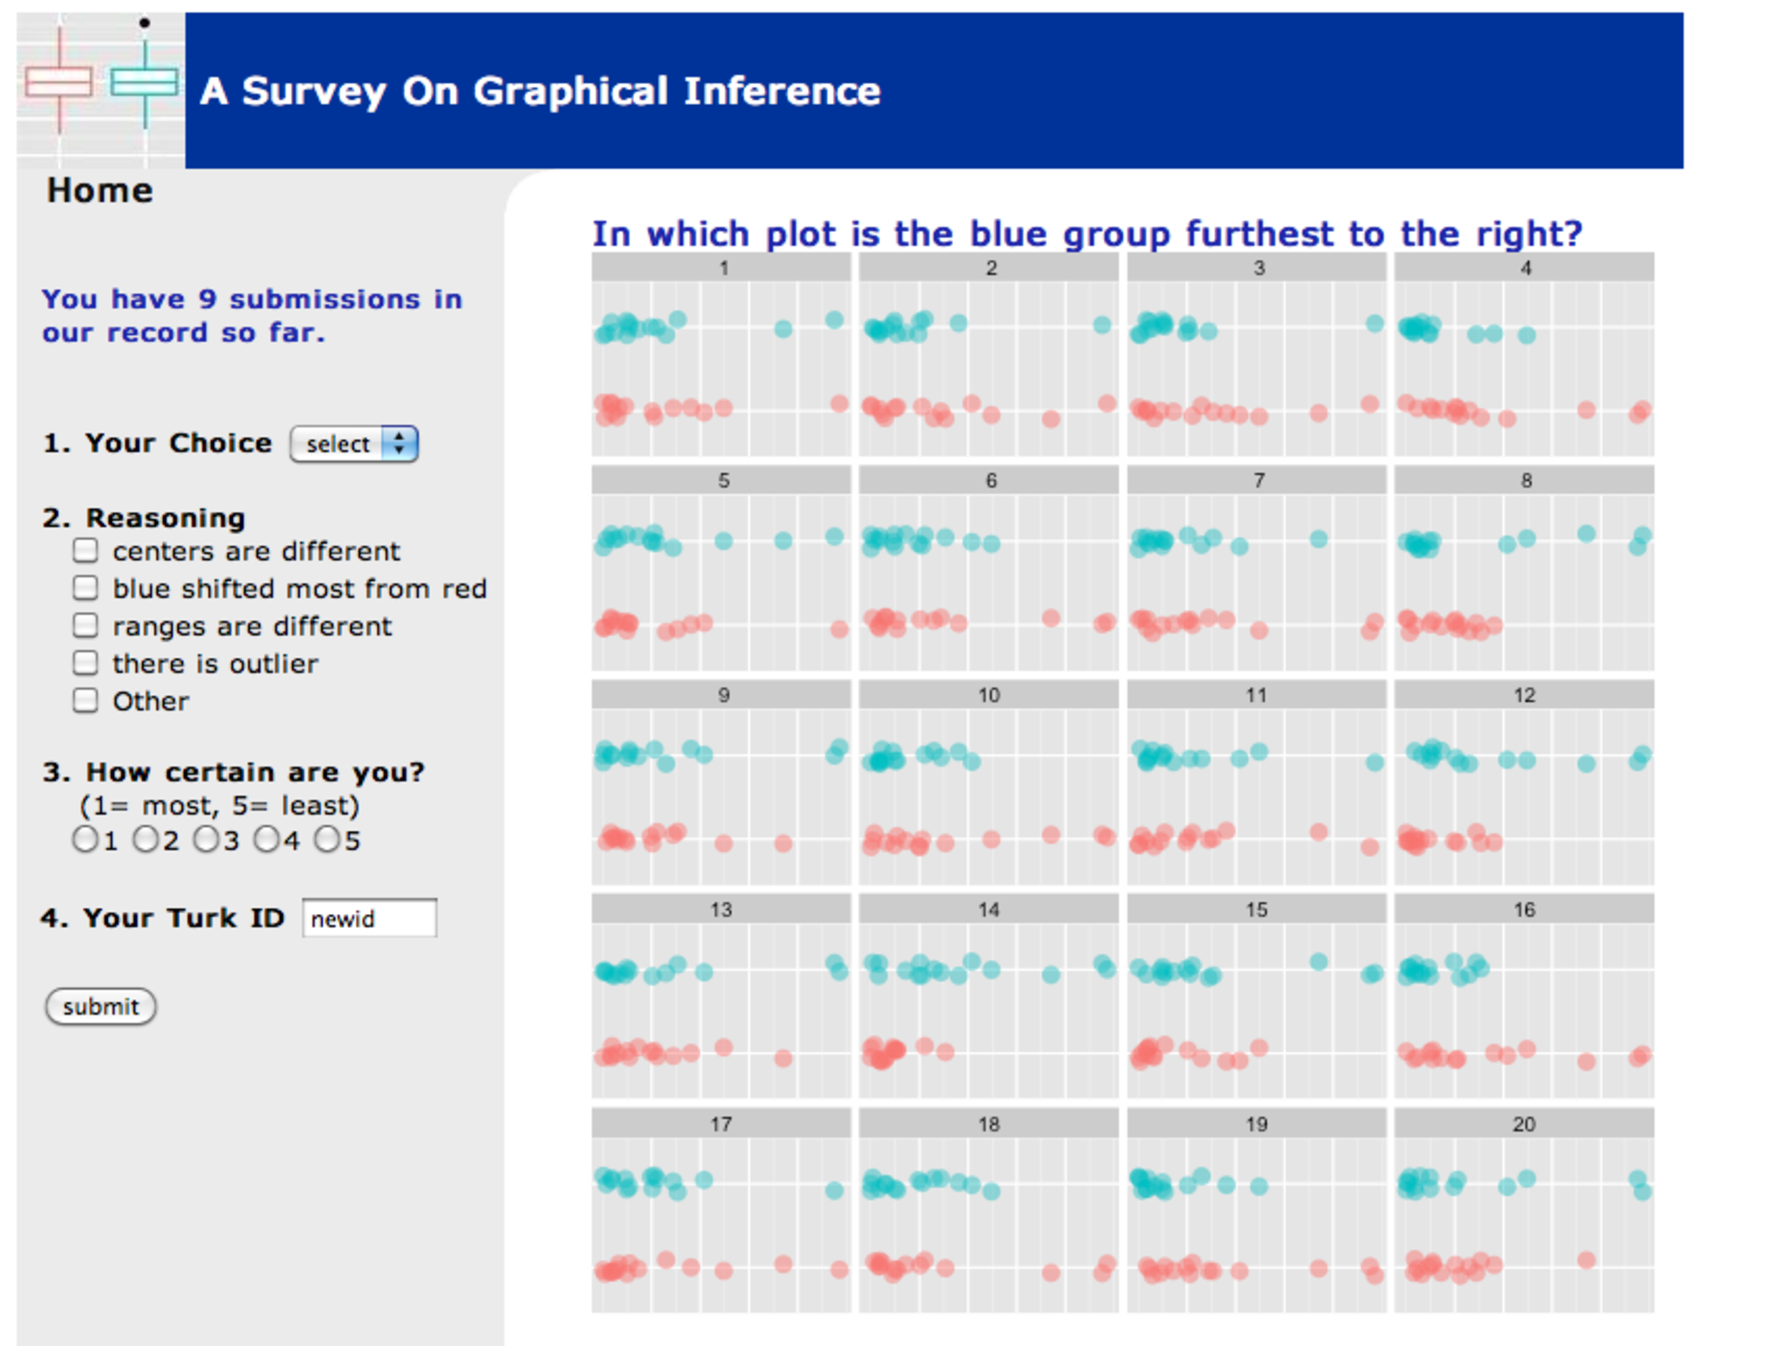
\includegraphics[width=\linewidth]{website} 
\vspace{-.2in}
   \caption{Screenshot of the website for the second study. }
   \label{fig:screen}
\end{figure}

Each participant is shown ten lineups and asked to identify the plot that is the most different from the other plots. In the second study the `difference' is further specified as `In which plot is the blue group the furthest to the right?". 
 In both studies, though, the question is placed prominently above each lineup as a reminder of what participants are asked to look for.  Additionally, participants are asked for a reason for their choice. They can select from a list of choices particular to the lineup design, why they chose this particular plot as well as how confident they are on a scale of one to five, where higher values indicate higher confidence. Personal information on age group, gender, and education is collected on a voluntary basis.  The amount of time it takes the individual to answer is also recorded.  This  allows us to assess how design choices affect decoding \cite{cleveland:1994} in terms of accuracy and speed.
 
 In order to avoid people `gaming the system' as found in earlier studies \cite{heer:2010, kosara:2010}, two of the ten lineups participants were shown were specially prepared as a baseline of performance -- if participants fail to answer some of these baseline lineups, we require at least two correct answers for the remaining plots, which is indicative of a better-than-guessing performance, as inclusion criterion for the data evaluation. 

